\documentclass[11pt,a4paper]{article}
\usepackage[top=3cm, bottom=2cm, left=3cm, right=2cm]{geometry}
\usepackage[utf8]{inputenc}
\usepackage{amsmath, amsfonts, amssymb}
\usepackage[brazil]{babel}
\usepackage[dvipsnames, svgnames]{xcolor}
\usepackage{tcolorbox}
\usepackage{tikz}
\usepackage{LobsterTwo}
\usepackage[T1]{fontenc}
\usepackage{fontspec}
\usepackage{txfonts}
\usepackage{titlesec}

\usepackage{lipsum}

\usetikzlibrary{patterns}
\tcbuselibrary{breakable}

\tcbuselibrary{raster}
\tcbuselibrary{skins}
\tcbuselibrary{listings}
\tcbuselibrary{theorems}
\tcbuselibrary{hooks}
\tcbuselibrary{vignette}

\newsavebox\mysavebox

\titleformat{\tilte}{\LobsterTwo\LARGE\color{CarnationPink}}{\thetitle}{1em}{}
\titleformat{\section}{\LobsterTwo\LARGE\color{CarnationPink}}{\thesection}{1em}{}
\titleformat{\subsection}{\LobsterTwo\LARGE\color{CarnationPink}}{\thesubsection}{1em}{}

\title{\textcolor{CarnationPink}{\LobsterTwo\Huge{Mapa Mental}}}
\author{Dalila}
\date{}
\begin{document}
    \maketitle
\section{Box}
    \begin{tcboxedraster}[raster columns=3, raster equal height,
        size=small,colframe=red!50!black,colback=red!10!white,colbacktitle=red!50!white,
        title={Box \# \thetcbrasternum}]
        {colback=yellow!10,fonttitle=\bfseries,title=Boxed Raster}
        \begin{tcolorbox}First box\end{tcolorbox}
        \begin{tcolorbox}Second box\end{tcolorbox}
        \begin{tcolorbox}This is a box\\with a second line\end{tcolorbox}
        \begin{tcolorbox}Another box\end{tcolorbox}
        \begin{tcolorbox}A box again\end{tcolorbox}
        \end{tcboxedraster}

\section{Multilinhas}

        \begin{tcbitemize}[raster rows=3,raster columns=3,raster height=6cm,
            raster every box/.style={colframe=red!50!black,colback=red!10!white}]
            \tcbitem ahahah
            \tcbitem HhH
            \tcbitem AHAHAH
            \tcbitem[colframe=blue!50!black,colback=blue!10!white,raster multirow=2]
            multirow=2
            \tcbitem[raster multicolumn=2,raster multirow=2,blankest]
                \begin{tcbitemize}[raster rows=2,raster columns=2,raster height=\tcbtextheight]
                    \tcbitem
                    \tcbitem
                    \tcbitem
                    \tcbitem
                \end{tcbitemize}
        \end{tcbitemize}

\section{Muda cor de um Box}

        \begin{tcbitemize}[raster columns=2, raster equal height=rows,
            size=small,colframe=red!50!black,colback=red!10!white,colbacktitle=red!50!white,
            title={Box \# \thetcbrasternum}]
            \tcbitem First box
            \tcbitem Second box
            \tcbitem This is a box\\with a second line
            \tcbitem[colback=yellow,colbacktitle=yellow!50!black] Another box
            \tcbitem A box again
        \end{tcbitemize}

\section{Imagnes}

        \begin{tcbraster}[raster columns=3,raster force size=false,size=fbox,
            colframe=red!50!black,colback=red!20!black,
            fonttitle=\bfseries,center title,drop fuzzy shadow]
            \tcbincludegraphics[title=Normal]{goldshade.png}
            \tcbincludegraphics[title=Fixed height,height=3cm]{goldshade.png}
            \tcbincludegraphics[title=hbox mode,hbox,graphics options={width=3cm}]
            {goldshade.png}
        \end{tcbraster}

\section{Imagens}

        \begin{tcbraster}[size=fbox,
            colframe=red!50!black,colback=red!20!black,
            fonttitle=\bfseries\ttfamily,center title,drop fuzzy shadow]
            \tcbincludegraphics[title=\imagename]{goldshade.png}
            \tcbincludegraphics[finish={
            \node[fill=white,fill opacity=0.5,text opacity=1]
            at (frame.center) {\bfseries\ttfamily\imagename};}]{blueshade.png}
        \end{tcbraster}
            
\section{Tikz}

    \begin{tikzpicture}
        \draw[thick,rounded corners=8pt]
        (0,0) -- (0,2) -- (1,3.25) -- (2,2) -- (2,0)
        -- (0,2) -- (2,2) -- (0,0) -- (2,0);
        \tcbpatcharcangular
        \draw[thick,rounded corners=8pt,xshift=2.5cm]
        (0,0) -- (0,2) -- (1,3.25) -- (2,2) -- (2,0)
        -- (0,2) -- (2,2) -- (0,0) -- (2,0);
        \end{tikzpicture}

\section{Firula}

\begin{tikzpicture}
    \node[draw,fill=blue!15!white] (A) {Another Test};
    \tcbvignette{size=3mm,outside node=A,
    north style=red,east style=yellow,
    south style=blue,west style=green}
\end{tikzpicture}

\begin{tikzpicture}
    \node[fill=yellow!10] (A) {\LobsterTwo\Large{Mapa Mental}};
    \tcbvignette{size=4mm,outside node=A,
    north style=CarnationPink,east style=DarkTurquoise,
    south style=Melon,west style=MediumOrchid}
\end{tikzpicture}


\section{Outra Multicoluna}

\begin{tcbitemize}[raster equal height=rows,raster columns=3,
    title=\thetcbrasternum,colframe=red!50!black,colback=red!10!white]
    \tcbitem[colframe=blue!50!black,colback=blue!10!white,raster multicolumn=1]
    multicolumn=1
    \tcbitem
    \tcbitem
    \tcbitem[colframe=blue!50!black,colback=blue!10!white,raster multicolumn=2]
    multicolumn=2
    \tcbitem
    \tcbitem[colframe=blue!50!black,colback=blue!10!white,raster multicolumn=3]
    multicolumn=3
    \tcbitem
    \tcbitem[colframe=blue!50!black,colback=blue!10!white,raster multicolumn=2]
    multicolumn=2
    \end{tcbitemize}




    
\section{Babozeira com Figura}



\begin{tcolorbox}[colframe=blue!75!black,colback=white,height=3cm,
    space to=\myspace]
    This is my box of height 3cm. The space is filled with a picture:\\[2mm]
    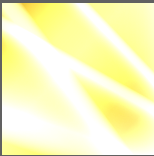
\includegraphics[width=\linewidth,height=\myspace]{goldshade.png}\\[1mm]
    This is some other text.
    \end{tcolorbox}



\section{Firulaa}

\newtcolorbox{mybox}[2][]{colback=red!5!white,
colframe=red!75!black,fonttitle=\bfseries,
colbacktitle=red!85!black,enhanced,
attach boxed title to top center={yshift=-2mm},
title={#2},#1}
\begin{mybox}[colback=yellow]{Hello there}
This is my own box with a mandatory title
and options.
\end{mybox}

\section{itemizxee}

\newenvironment{myitemize}{%
\begin{itemize}}{\end{itemize}}
\tcolorboxenvironment{myitemize}{blanker,
before skip=6pt,after skip=6pt,
borderline west={0.2mm}{0pt}{red}}
Some text.
\begin{myitemize}
\item Alpha
\item Beta
\item Gamma
\end{myitemize}
More text.


\section{Outra subtitulo}

\begin{tcolorbox}[title=My title,
    colback=red!5!white,
    colframe=red!75!black,
    colbacktitle=yellow!50!red,
    coltitle=red!25!black,
    fonttitle=\bfseries,
    subtitle style={boxrule=0.4pt,
    colback=yellow!50!red!25!white,
    colupper=red!75!gray} ]
    This is a \textbf{tcolorbox}.
    \tcbsubtitle{My subtitle}
    Further text.
    \tcbsubtitle{Second subtitle}
    Further text.
    \end{tcolorbox}
    
\section{Outro texto}

\newtcolorbox{mybox2}[2][]{colbacktitle=red!10!white,
    colback=blue!10!white,coltitle=red!70!black,
    title={#2},fonttitle=\bfseries,#1}
    
    \begin{mybox2}{My title}
        This is a \textbf{tcolorbox}.
        \end{mybox2}
        \begin{mybox2}[detach title,before upper={\tcbtitle\quad}]{My title}
        This is a \textbf{tcolorbox}.
        \end{mybox2}
        \begin{mybox2}[detach title,after upper={\par\hfill\tcbtitle}]{My title}
        This is a \textbf{tcolorbox}.
        \end{mybox2}

\section{Reparticoes}
        
\begin{tcolorbox}[saveto=\jobname_mysave2.tex]
This is a \textbf{tcolorbox}.
\tcblower
This is the lower part.
\end{tcolorbox}
Now, we load the saved text:
\begin{tcolorbox}[colframe=red,colback=red!10,
coltitle=black,colbacktitle=red!20,sidebyside,
title=Here we see the saved content including the lower part]
\input{\jobname_mysave2.tex}
\end{tcolorbox}


\section{Alinhamentos}

\tcbset{colback=red!5!white,colframe=red!75!black,size=small,
fonttitle=\bfseries,width=3.5cm,box align=top,
nobeforeafter}
\begin{tcolorbox}[adjusted title=flush center,halign=flush center]
This is a demonstration text for showing how line breaking works.
\end{tcolorbox}
\begin{tcolorbox}[adjusted title=flush left,halign=flush left]
This is a demonstration text for showing how line breaking works.
\end{tcolorbox}
\begin{tcolorbox}[adjusted title=flush right,halign=flush right]
This is a demonstration text for showing how line breaking works.
\end{tcolorbox}
\begin{tcolorbox}[adjusted title=center,halign=center]
This is a demonstration text for showing how line breaking works.
\end{tcolorbox}
\begin{tcolorbox}[adjusted title=left,halign=left]
This is a demonstration text for showing how line breaking works.
\end{tcolorbox}
\begin{tcolorbox}[adjusted title=right,halign upper=right]
This is a demonstration text for showing how line breaking works.
\end{tcolorbox}


\section{Bordas}

\tcbset{colback=red!5!white,colframe=red!75!black}
\begin{tcolorbox}[toprule=3mm]
This is a \textbf{tcolorbox}.
\end{tcolorbox}

\begin{tcolorbox}[bottomrule=3mm]
    This is a \textbf{tcolorbox}.
    \end{tcolorbox}


\begin{tcolorbox}[leftrule=3mm]
This is a \textbf{tcolorbox}.
\end{tcolorbox}

\begin{tcolorbox}[rightrule=3mm]
    This is a \textbf{tcolorbox}.
    \end{tcolorbox}


\section{Formas}

\begin{tcolorbox}[width=3cm,
    colback=red!5!white,
    colframe=red!75!black,
    halign=center,valign=center,
    square,circular arc]
    This is a \textbf{tcolorbox}.
\end{tcolorbox}

    \tcbset{size=fbox,boxrule=0.5mm,
    colback=red!5!white,
    colframe=red!75!black,
    halign=center,valign=center}
    \begin{tcolorbox}[width=3cm,height=2cm,
    bean arc]
    Box A
    \end{tcolorbox}
    \begin{tcolorbox}[width=2cm,height=3cm,
    bean arc]
    Box B
    \end{tcolorbox}


    \begin{tcolorbox}[enhanced,
        size=minimal,auto outer arc,
        width=2.1cm,octogon arc,
        colback=red,colframe=white,colupper=white,
        fontupper=\fontsize{7mm}{7mm}\selectfont\bfseries\sffamily,
        halign=center,valign=center,
        square,arc is angular,
        borderline={0.2mm}{-1mm}{red} ]
        STOP
        \end{tcolorbox}
        
\section{Tamanhos}

% \tcbset{colback=red!5!white,colframe=red!75!black,fonttitle=\bfseries}
% \textit{Normal text for comparison:}\\
% \lipsum[2]
% \begin{tcolorbox}[oversize,title=Oversized box]
% \lipsum[2]
% \end{tcolorbox}
% \begin{tcolorbox}[title=Normal box]
% \lipsum[2]
% \end{tcolorbox}


% \begin{tcolorbox}[enhanced,breakable,
%     toggle left and right,sharp corners,
%     boxrule=0mm,top=0mm,bottom=0mm,left=1mm,right=1mm,
%     rightrule=1cm,colupper=blue!25!black,
%     interior style={fill overzoom image=lichtspiel.jpg,fill image opacity=0.25},
%     frame style={pattern=crosshatch dots light steel blue},
%     overlay={%
%     \begin{tcbclipframe}
%     \tcbifoddpage{\coordinate (X) at ([xshift=-5mm]frame.east);}
%     {\coordinate (X) at ([xshift=5mm]frame.west);}
%     \fill[shading=ball,ball color=blue!50!white,opacity=0.5] (X) circle (4mm);
%     \end{tcbclipframe}}]
%     \lipsum[1-6]
%     \end{tcolorbox}


    \begin{tcolorbox}[standard jigsaw,colframe=red,
        opacityfill=0.7, title=This is a title]
        This is a \textbf{tcolorbox}.
        \end{tcolorbox}


        \tcbset{frogbox/.style={enhanced,colback=green!10,colframe=green!65!black,
        enlarge top by=5.5mm,
        overlay={\foreach \x in {2cm,3.5cm} {
        \begin{scope}[shift={([xshift=\x]frame.north west)}]
        \path[draw=green!65!black,fill=green!10,line width=1mm] (0,0) arc (0:180:5mm);
        \path[fill=black] (-0.2,0) arc (0:180:1mm);
        \end{scope}}}}}
        \begin{tcolorbox}[frogbox,title=My title]
        This is a \textbf{tcolorbox}.
        \end{tcolorbox}
        

        \newtcolorbox[blend into=figures]{myfigure}[2][]{float=htb,capture=hbox,
        blend before title code={\fbox{##1}\ },title={#2},every float=\centering,#1}
        \begin{myfigure}{A tcolorbox figure}
        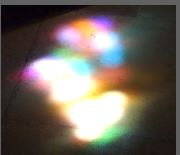
\includegraphics[height=6cm]{lichtspiel.jpg}
        \end{myfigure}


        % \begin{tcolorbox}[bicolor,sidebyside,righthand width=3cm,
        %     sharp corners,boxrule=.4pt,colback=green!5,colbacklower=green!50!black!50]
        %     \lipsum[2]
        %     \tcblower
        %     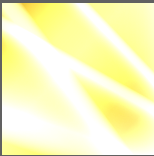
\includegraphics[width=\linewidth]{goldshade}%
        % \end{tcolorbox}
            

        % \DeclareTotalTColorBox{\mysidebox}{ O{} +m +m }{
        %     bicolor,colback=white,colbacklower=yellow!10,
        %     fonttitle=\bfseries,center title,
        %     sidebyside,
        %     code={\sbox{\mysavebox}{#2}},
        %     lefthand width=\wd\mysavebox,
        %     drop lifted shadow,
        %     #1
        %     }
        %     {\usebox{\mysavebox}\tcblower#3}
        %     \mysidebox[title=The Triangle]{%
        %     \begin{tikzpicture}
        %     \path[fill=red!20,draw=red!50!black]
        %     (0,0) node[below]{A} -- (3,1) node[right]{B}
        %     -- (1,4) node[above]{C} -- cycle;
        %     \end{tikzpicture}%
        %     }{%
        %     \lipsum[1]
        %     }
    

            \begin{tcolorbox}[enhanced,frame code={
                \foreach \n in {north east,north west,south east,south west}
                {\path [fill=red!75!black] (interior.\n) circle (3mm); } }]
                This is a \textbf{tcolorbox}.
                \tcblower
                This is the lower part.
                \end{tcolorbox}

\section{Seo}

\tcbset{colback=red!5!white,fonttitle=\bfseries}
\begin{tcolorbox}[enhanced,title=My title,
frame style={left color=red!75!black,
right color=blue!75!black}]
This is a \textbf{tcolorbox}.
\tcblower
This is the lower part.
\end{tcolorbox}

\section{sss}

\newtcolorbox{mybox3}[1][]{enhanced,
fuzzy shadow={1.0mm}{-1.0mm}{0.12mm}{0mm}{blue!50!white},
fuzzy shadow={-1.0mm}{-1.0mm}{0.12mm}{0mm}{red!50!white},
fuzzy shadow={-1.0mm}{1.0mm}{0.12mm}{0mm}{green!50!white},
fuzzy shadow={1.0mm}{1.0mm}{0.12mm}{0mm}{yellow!50!white},#1
}
\begin{mybox3}[title=A multi shadow box]
This is a tcolorbox.
\end{mybox3}

\section{sombra}

\tcbset{enhanced,colback=red!5!white,
colframe=red!75!black,fonttitle=\bfseries}
\begin{tcolorbox}[title=My own shadow,
fuzzy shadow={2mm}{-1mm}{0mm}{0.1mm}%
{black!50!white}]
This is a tcolorbox.
\end{tcolorbox}
\par\bigskip
\begin{tcolorbox}[title=Another shadow,
fuzzy shadow={-1mm}{-2mm}{0mm}{0.2mm}%
{fill=blue}]
This is a tcolorbox.
\end{tcolorbox}
\par\bigskip
\begin{tcolorbox}[title=Double shadow,
fuzzy shadow={-1.5mm}{-1.5mm}{0mm}{0.1mm}%
{blue},
fuzzy shadow={1.5mm}{-1.5mm}{0mm}{0.1mm}%
{red}]
This is a tcolorbox.
\end{tcolorbox}
\par\bigskip
\begin{tcolorbox}[title=Far shadow,
fuzzy shadow={5.5mm}{-3.5mm}{0mm}{0.3mm}%
{black}]
This is a tcolorbox.
\end{tcolorbox}
\par\bigskip\bigskip
\begin{tcolorbox}[title=Glow shadow,
fuzzy shadow={0mm}{0mm}{-1.5mm}{0.15mm}%
{yellow!75!red}]
This is a tcolorbox.
\end{tcolorbox}

\section{Math}

\tcbset{myformula/.style={colback=yellow!10!white,colframe=red!50!black,
every box/.style={highlight math style={colback=LightBlue!50!white,colframe=Navy}}
}}
\begin{align}
\tcbhighmath{\sum\limits_{n=1}^{\infty} \frac{1}{n}} &= \infty.\\
\int x^2 ~\text{d}x &= \frac13 x^3 + c.
\end{align}
\begin{tcolorbox}[ams align,myformula]
\tcbhighmath{\sum\limits_{n=1}^{\infty} \frac{1}{n}} &= \infty.\\
\int x^2 ~\text{d}x &= \frac13 x^3 + c.
\end{tcolorbox}


\section{Mathdffa}

\tcbset{frogbox/.style={enhanced,colback=green!10,colframe=green!65!black,
enlarge top by=5.5mm,
overlay={\foreach \x in {2cm,3.5cm} {
\begin{scope}[shift={([xshift=\x]frame.north west)}]
\path[draw=green!65!black,fill=green!10,line width=1mm] (0,0) arc (0:180:5mm);
\path[fill=black] (-0.2,0) arc (0:180:1mm);
\end{scope}}}}}
\tcbset{ribbon/.style={overlay app={%
\path[fill=blue!75!white,draw=blue,double=white!85!blue,
preaction={opacity=0.6,fill=blue!75!white},
line width=0.1mm,double distance=0.2mm,
pattern=fivepointed stars,pattern color=white!75!blue]
([xshift=-0.2mm,yshift=-1.02cm]frame.north east)
-- ++(-1,1) -- ++(-0.5,0) -- ++(1.5,-1.5) -- cycle;}}}
\begin{tcolorbox}[frogbox,title=My title]
This is a \textbf{tcolorbox}.
\end{tcolorbox}
\begin{tcolorbox}[frogbox,ribbon,title=My title]
This is a \textbf{tcolorbox}.\par
Here, we apply a second overlay.
\end{tcolorbox}


\end{document}